\section{载流子浓度}
现在让我们回到本章的中心问题,即载流子浓度的计算,根据\xref{sec:状态密度}\setpeq{载流子浓度}
\begin{Equation}&[1]
    \dd{Z}=g_\text{c}(E)\dd{E}
\end{Equation}
这里$\dd{Z}$是$E$至$E+\dd{E}$的量子态,这些量子态上未必有电子,根据\xref{sec:费米分布与玻尔兹曼分布},非简并半导体的电子遵从玻尔兹曼分布$f(E)$,因而$f(E)\dd{Z}$就是$E$至$E+\dd{E}$的电子数目,记为
\begin{Equation}&[2]
    \dd{N}=f(E)g_\text{c}(E)\dd{E}
\end{Equation}
而电子的能量并不影响电子的记数,所以我们只需要将$\dd{N}$在导带的能量区间上积分,就可以得到导带上的电子数目,这样一来,只要将求得的数目除以晶体体积,就可以得到电子浓度。

\subsection{导带电子浓度}
现在让我们来实践上面的思路,不过还是有些麻烦的,原因是积分略微有些复杂。
\begin{BoxFormula}[导带电子浓度]
    导带电子浓度满足
    \begin{Equation}&[A]
        n_0=N_\text{c}\exp(\frac{E_\text{F}-E_\text{c}}{\kB T})=N_\text{c}f(E_\text{c})
    \end{Equation}
    其中$N_\text{c}$称为导带的有效状态密度,满足
    \begin{Equation}&[B]
        N_\text{c}=2\qty(\frac{\mne\kB T}{2\pi\hbar^2})^{3/2}
    \end{Equation}
\end{BoxFormula}
\begin{Proof}
    我们从\xrefpeq[载流子浓度]{2}出发,引入$\dd{n}$作为$E$至$E+\dd{E}$间的电子浓度
    \begin{Equation}&[1]
        \dd{n}=\frac{\dd{N}}{V}=\frac{f(E)g_\text{c}(E)\dd{E}}{V}
    \end{Equation}
    根据\fancyref{fml:导带底的状态密度}和\fancyref{fml:玻尔兹曼分布}
    \begin{Equation}&[2]
        \dd{n}=\frac{1}{V}\qty[\frac{V}{2\pi^2}\frac{(2\mne)^{3/2}}{\hbar^3}(E-E_\text{c})^{1/2}]\qty[\exp(\frac{E_\text{F}-E}{\kB T})]
    \end{Equation}
    将$V$约掉,并对指数部分做一些调整
    \begin{Equation}&[3]
        \dd{n}=\frac{1}{2\pi^2}\frac{(2\mne)^{3/2}}{\hbar^3}(E-E_\text{c})^{1/2}\exp(\frac{E_\text{F}-E_\text{c}}{\kB T})\exp(\frac{E_\text{c}-E}{\kB T})
    \end{Equation}
    现在,让我们对$\dd{n}$进行积分
    \begin{Equation}&[4]
        \qquad\qquad
        n_0=\frac{1}{2\pi^2}\frac{(2\mne)^{3/2}}{\hbar^3}\exp(\frac{E_\text{F}-E_\text{c}}{\kB T})\Int[E_\text{c}][E_\text{c}']\exp(\frac{E_\text{c}-E}{\kB T})(E-E_\text{c})^{1/2}\dd{E}
        \qquad\qquad
    \end{Equation}
    这里$n_0$即电子浓度,$E_\text{c}$是导带底,$E_\text{c}'$是导带上限,如果我们引入$x=(E-E_\text{c})/\kB T$的代换,我们注意到$\dd{E}=k_0T\dd{x}$,并且,当$E=E_\text{c}$时有$x=0$,当$E=E_\text{c}'$姑且记$x=x'$
    \begin{Equation}&[5]
        n_0=\frac{1}{2\pi^2}\frac{(2\mne)^{3/2}}{\hbar^3}\exp(\frac{E_\text{F}-E_\text{c}}{\kB T})\Int[0][x']\e^{-x}(\kB T x)^{1/2}\kB T\dx
    \end{Equation}
    提出与积分无关的常数
    \begin{Equation}&[6]
        n_0=\frac{1}{2\pi^2}\frac{(2\mne)^{3/2}}{\hbar^3}(\kB T)^{3/2}\exp(\frac{E_\text{F}-E_\text{c}}{\kB T})\Int[0][x']x^{1/2}\e^{-x}\dx
    \end{Equation}
    由此可见,求解的关键就在于这个积分的计算,我们姑且将其记为$I$
    \begin{Equation}&[7]
        I=\Int[0][x']x^{1/2}\e^{-x}\dd{x}
    \end{Equation}
    遗憾的是,此处的被积函数$x^{1/2}\e^{-x}$的原函数是非初等的,但是,作为物理问题,我们可以采用一些近似手段,如\xref{fig:根号负指数函数的图像}所示,函数$x^{1/2}\e^{-x}$随着$x$增大,会先增大,然后迅速趋于零。
    \begin{Figure}[函数$x^{1/2}\e^{-x}$的图像;根号负指数函数的图像]
        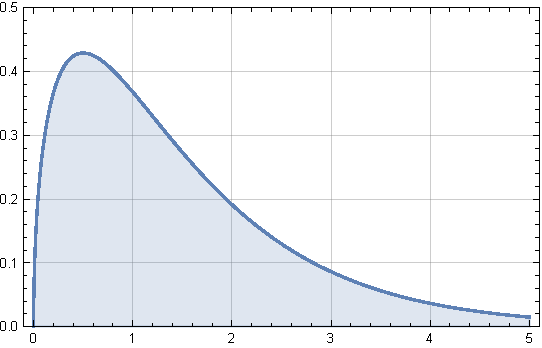
\includegraphics{Mathematica/output/SqrtExp.pdf}
    \end{Figure}
    因此,如果我们将\xrefpeq{7}的积分上限由$x'$改为$\infty$,并不会有太大的误差
    \begin{Equation}&[8]
        I=\Int[0][\infty]x^{1/2}\e^{-x}\dd{x}
    \end{Equation}
    而转化为无穷后,我们就可以将其向高斯积分的方向转化了,令$t=x^{1/2}$,则$\dd{x}=2t\dd{t}$
    \begin{Equation}&[9]
        I=2\Int[0][\infty]t^2\e^{-t^2}\dd{t}
    \end{Equation}
    而高斯积分的结论告诉我们
    \begin{Equation}&[10]
        I=2\frac{\sqrt{\pi}}{4}=\frac{\sqrt{\pi}}{2}
    \end{Equation}
    将\xrefpeq{10}代入\xrefpeq{6}
    \begin{Equation}&[11]
        n_0=\frac{1}{4\pi^{3/2}}\frac{(2\mne)^{3/2}}{\hbar^3}(\kB T)^{3/2}\exp(\frac{E_\text{F}-E_\text{c}}{\kB T})
    \end{Equation}
    我们可以将系数整理为一个统一的$3/2$次项
    \begin{Equation}&[12]
        n_0=\frac{1}{4}\qty(\frac{2\mne\kB T}{\pi\hbar^2})^{3/2}\exp(\frac{E_\text{F}-E_\text{c}}{\kB T})
    \end{Equation}
    我们在系数的括号内除以$4$,这相当于在括号外要乘$4^{3/2}=8$
    \begin{Equation}&[13]
        n_0=2\qty(\frac{\mne\kB T}{2\pi\hbar^2})^{3/2}\exp(\frac{E_\text{F}-E_\text{c}}{\kB T})
    \end{Equation}
    若记\xrefpeq{13}左端的常系数为$N_\text{c}$,我们就可以得到\xrefpeq{A}的结论形式,而依据\fancyref{fml:玻尔兹曼分布},此时\xrefpeq{13}右端的指数项$\exp(E_\text{F}-E_\text{c}/\kB T)$,其实也可以记为$f(E_\text{c})$。
\end{Proof}

\subsection{价带空穴浓度}
\begin{BoxFormula}[价带空穴浓度]
    价带空穴浓度满足
    \begin{Equation}&[A]
        p_0=N_\text{v}\exp(\frac{E_\text{v}-E_\text{F}}{\kB T})=N_\text{v}[1-f(E_\text{v})]
    \end{Equation}
    其中$N_\text{v}$称为价带的有效状态密度,满足
    \begin{Equation}&[B]
        N_\text{v}=2\qty(\frac{\mpe\kB T}{2\pi\hbar^2})^{3/2}
    \end{Equation}
\end{BoxFormula}

\begin{Proof}
    我们仍然从\xrefpeq[载流子浓度]{2}出发,但是这一次$f(E)$需要更换为$1-f(E)$,而$g_\text{c}(E)$需要换为$g_\text{v}(E)$
    \begin{Equation}&[1]
        \dd{n}=\frac{\dd{N}}{V}=\frac{[1-f(E)]g_\text{v}(E)}{V}
    \end{Equation}
    根据\fancyref{fml:价带顶的状态密度}和\fancyref{fml:玻尔兹曼分布}
    \begin{Equation}&[2]
        \dd{n}=\frac{1}{V}\qty[\frac{V}{2\pi^3}\frac{(2\mpe)^{3/2}}{\hbar^3}(E_\text{v}-E)^{1/2}]\qty[\exp(\frac{E-E_\text{F}}{\kB T})]
    \end{Equation}
    将$V$约掉,并对指数部分做一些调整
    \begin{Equation}&[3]
        \dd{n}=\frac{1}{2\pi^2}\frac{(2\mpe)^{3/2}}{\hbar^3}(E_\text{v}-E)^{1/2}\exp(\frac{E_\text{v}-E_\text{F}}{\kB T})\exp(\frac{E-E_\text{v}}{\kB T})
    \end{Equation}
    现在,让我们对$\dd{n}$进行积分
    \begin{Equation}&[4]
        \qquad\qquad
        p_0=\frac{1}{2\pi^2}\frac{(2\mpe)^{3/2}}{\hbar^3}\exp(\frac{E_\text{v}-E_\text{F}}{\kB T})\Int[E_\text{v}'][E_\text{v}]\exp(\frac{E-E_\text{v}}{\kB T})(E_\text{v}-E)^{1/2}\dd{E}
        \qquad\qquad
    \end{Equation}
    后续的步骤是完全相似的,积分后化简为
    \begin{Equation}&[5]
        p_0=2\qty(\frac{\mpe\kB T}{2\pi\hbar^2})^{3/2}\exp(\frac{E_\text{v}-E_\text{F}}{\kB T})
    \end{Equation}
    若记\xrefpeq{5}左端的常系数为$N_\text{v}$,我们就可以得到\xrefpeq{A}的结论形式,而依据\fancyref{fml:玻尔兹曼分布},此时\xrefpeq{5}右端的指数项$\exp(E_\text{v}-E_\text{F}/\kB T)$,其实亦可记为$1-f(E_\text{v})$。
\end{Proof}

\subsection{载流子的浓度乘积}
\begin{BoxFormula}[载流子的浓度乘积]
    载流子的浓度乘积满足
    \begin{Equation}
        n_0p_0=N_\text{c}N_\text{v}\exp(-\frac{E_\text{g}}{\kB T})
    \end{Equation}
    或者展开$N_\text{c},N_\text{v}$
    \begin{Equation}
        n_0p_0=4T^3\qty(\mne\mpe)^{3/2}\qty(\frac{\kB}{2\pi\hbar^2})^3\exp(-\frac{E_\text{g}}{\kB T})
    \end{Equation}
\end{BoxFormula}
\begin{Proof}
    这很容易证明,根据\fancyref{fml:导带电子浓度}和\fancyref{fml:价带空穴浓度}
    \begin{Equation}&[1]
        n_0p_0=N_\text{c}N_\text{v}\exp(\frac{E_\text{F}-E_\text{c}}{\kB T})\exp(\frac{E_\text{v}-E_\text{F}}{\kB T})
    \end{Equation}
    合并两个指数项
    \begin{Equation}&[2]
        n_0p_0=N_\text{c}N_\text{v}\exp(\frac{E_\text{v}-E_\text{c}}{\kB T})
    \end{Equation}
    我们知道禁带宽度$E_\text{g}=E_\text{c}-E_\text{v}$
    \begin{Equation}*
        n_0p_0=N_\text{c}N_\text{v}\exp(-\frac{E_\text{g}}{\kB T})\qedhere
    \end{Equation}
\end{Proof}

\fancyref{fml:载流子的浓度乘积}告诉我们一个重要的事实,\empx{电子和空穴的浓度乘积与费米能级无关}。该结论普遍适用于一切热平衡状态下的非简并半导体,且对本征半导体和杂质半导体都成立。实际上,掺杂改变的主要就是费米能级,故对于某种半导体材料,掺杂与否,掺杂的多少,并不会改变$n_0p_0$的结果,这会为我们之后讨论杂质半导体带来很多便利,比如
\begin{itemize}
    \item 如果掺杂使得电子浓度增加,那么空穴浓度必然会减少。
    \item 如果掺杂使得空穴浓度增加,那么空穴浓度必然会减少。
\end{itemize}
该结论还指出$n_0p_0$大致正比于$T^3$(在$T$较大时$\exp(-E_\text{g}/\kB T)$将趋向于$1$),这就表明,载流子的浓度乘积会随着温度增加而迅速增加,换言之,温度对于半导体的导电性的影响很大。